Die Funktion
\[
\varphi(x)=\begin{cases}
0&\qquad x< -1\\
\frac34(1-x^2)&\qquad -1\le x\le 1\\
0&\qquad x > 1
\end{cases}
\]
\begin{figure}[h]
\centering
\def\h{2.5}
\definecolor{darkred}{rgb}{0.8,0,0}
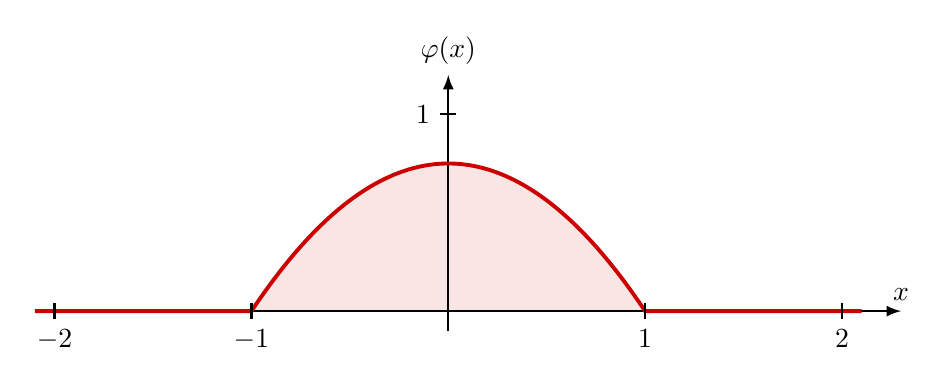
\begin{tikzpicture}[>=latex,thick]
\fill[color=darkred!10] 
	plot[domain=-1:1,samples=100] ({\x*\h},{\h*3*(1-\x*\x)/4})
		-- (\h,0) -- (-\h,0) -- cycle;
\draw[->] ({-2.1*\h},0) -- ({2.3*\h},0) coordinate[label={$x$}];
\draw[->] (0,{-0.1*\h}) -- (0,{1.2*\h}) coordinate[label={$\varphi(x)$}];
\draw[color=darkred,line width=1.4pt] ({-2.1*\h},0) -- (-\h,0) --
	plot[domain=-1:1,samples=100] ({\x*\h},{\h*3*(1-\x*\x)/4})
	-- (\h,0) -- ({2.1*\h},0);
\foreach \x in {-2,-1,1,2}{
	\draw ({\x*\h},-0.1) -- ({\x*\h},0.1);
	\node at ({\x*\h},-0.1) [below] {$\x$};
}
\draw (-0.1,\h) -- (0.1,\h);
\node at (-0.1,\h) [left] {$1$};
\end{tikzpicture}
\caption{Wahrscheinlichkeitsdichte für Aufgabe~\ref{50000024}.
\label{50000024:dichte}}
\end{figure}
(Abbildung~\ref{50000024:dichte})
sei die Wahrscheinlichkeitsdichte der unabhängigen Zufallsvariablen
$X$ und $Y$.
\begin{teilaufgaben}
\item Berechnen Sie die Verteilungsfunktion von $X$.
\item Zeichnen Sie einen Graphen der Verteilungsfunktion.
\item Berechnen Sie die Wahrscheinlichkeit dafür, dass die Zufallsvariable
Werte zwischen $-\frac12$ und $\frac12$ annimmt.
\item Berechnen Sie Erwartungswert und Varianz von $X$.
\item Zeichnen Sie Erwartungswert und $\sqrt{\operatorname{var}(X)}$ in
einem Graphen von $\varphi(x)$ ein.
\item Berechnen Sie die Wahrscheinlichkeitsdichte von $X+Y$.
\end{teilaufgaben}

\thema{Wahrscheinlichkeitsdichte}
\thema{Verteilungsfunktion}
\thema{Erwartungswert}
\thema{Varianz}
\thema{Faltung}

\begin{hinweis}
Verwenden Sie für Teilaufgabe f) eine Computeralgebrasystem oder einen
entsprechenden Taschenrechner.
\end{hinweis}

\begin{loesung}
Wir kontrollieren, dass $\varphi$ wirklich eine Wahrscheinlichkeitsverteilung
ist:
\begin{align*}
\int_{-\infty}^{\infty}\varphi(x)\,dx
=
\int_{-1}^1 \frac34(1-x^2)\,dx
=
\frac34\left[
x-\frac13x^3
\right]_{-1}^1
=
\frac34\biggl(1-\frac13-(-1)+\frac13(-1)\biggr)
=
\frac34\cdot\frac43
=1.
\end{align*}
\begin{teilaufgaben}
\item Die Verteilungsfunktion ist Stammfunktion von $\varphi$, also kann man sie
durch Integrieren finden:
\begin{align*}
F(x)&=0&&\text{für $x < -1$}\\
F(x)&=1&&\text{für $x > 1$}\\
F(x)&=\int_{-\infty}^x\varphi(\xi)\,d\xi =\int_{-1}^x\frac34(1-\xi^2)\,d\xi
\\
&=
\frac34\left[
\xi -\frac13\xi^3
\right]_{-1}^x
=\frac34(x-\frac13x^3-(-1)+\frac13(-1))
\\
&=-\frac14x^3+\frac34x+\frac12&&\text{für $-1\le x\le 1$}
\end{align*}
\item Der Graph der Verteilungsfunktion ist in
Abbildung~\ref{50000024:verteilungsfunktion} dargestellt.
\begin{figure}
\centering
\def\h{2.5}
\begin{tikzpicture}[>=latex,thick]
\draw[line width=0.2pt] (0,\h) -- (\h,\h);
\draw[->] ({-2.1*\h},0) -- ({2.3*\h},0) coordinate[label={$x$}];
\draw[->] (0,{-0.1*\h}) -- (0,{1.2*\h}) coordinate[label={right:$F(x)$}];
\draw[color=darkgreen,line width=1.4pt] ({-2.1*\h},0) -- (-\h,0) --
	plot[domain=-1:1,samples=100]
		({\x*\h},{\h*(0.5+0.75*(\x)-0.25*(\x*\x*\x))})
	-- (\h,\h) -- ({2.1*\h},{\h});
\foreach \x in {-2,-1,1,2}{
	\draw ({\x*\h},-0.1) -- ({\x*\h},0.1);
	\node at ({\x*\h},-0.1) [below] {$\x$};
}
\draw (-0.1,\h) -- (0.1,\h);
\node at (-0.1,\h) [left] {$1$};
\end{tikzpicture}
%\includeagraphics[]{graph-3.pdf}
\caption{Graph der Verteilungsfunktion von Aufgabe~\ref{50000024}
\label{50000024:verteilungsfunktion}}
\end{figure}
\item Die gesuchte Wahrscheinlichkeit kann direkt mit der Verteilungsfunktion
bestimmt werden:
\begin{align*}
P\biggl(-\frac12<X\le \frac12\biggr)
&=
F\biggl(\frac12\biggr)-F\biggl(-\frac12\biggr)
=
-\frac14\cdot\frac18+\frac34\cdot\frac12+\frac12
+\frac14\cdot\biggl(-\frac18\biggr)-\frac34\cdot\biggl(-\frac12\biggr)-\frac12
\\
&=-\frac12\cdot\frac18+\frac32\cdot\frac12
=
-\frac1{16}+\frac{12}{16}
=
\frac{11}{16}.
\end{align*}
\item
Erwartungswert und Varianz können mit den Standardformeln gefunden 
werden:
\begin{align*}
E(X)&=
\int_{-\infty}^{\infty}x\varphi(x)\,dx=\int_{-1}^1x \frac34(1-x^2)\,dx
=\frac34\left[\frac12x^2-\frac14x^4\right]_{-1}^1
=0\\
\operatorname{var}(X)&=E(X^2)=
\int_{-\infty}^{\infty}x^2\varphi(x)\,dx=\int_{-1}^1x^2\frac34(1-x^2)\,dx
=\frac34\left[\frac13x^3-\frac15x^5\right]_{-1}^1\\
&=\frac34\left(\frac13-\frac15+\frac13-\frac15\right)
=\frac34\left(\frac23-\frac25\right)
=\frac32\cdot\frac{5-3}{15}=\frac15.
\end{align*}
\item 
Abbildung~\ref{50000024:exvarx} zeigt die Wahrscheinlichkeitsdichte
$\varphi(x)$ mit eingezeichnetem Erwartungswert $E(X)$ und Varianz.
\begin{figure}
\centering
\def\h{2.5}
\definecolor{darkred}{rgb}{0.8,0,0}
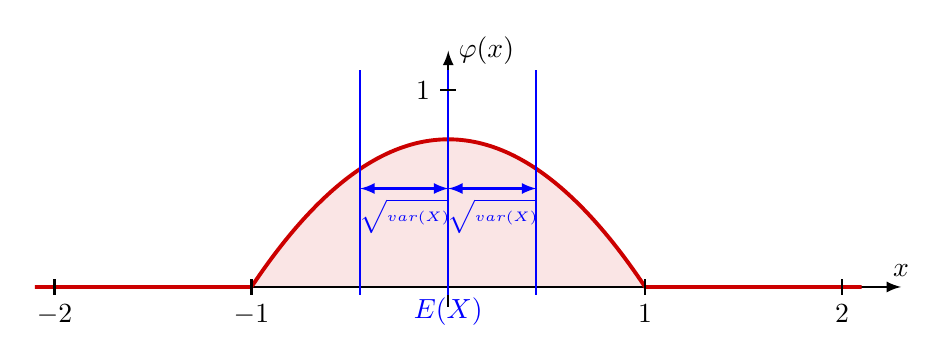
\begin{tikzpicture}[>=latex,thick]
\fill[color=darkred!10] 
	plot[domain=-1:1,samples=100] ({\x*\h},{\h*3*(1-\x*\x)/4})
		-- (\h,0) -- (-\h,0) -- cycle;
\draw[->] ({-2.1*\h},0) -- ({2.3*\h},0) coordinate[label={$x$}];
\draw[->] (0,{-0.1*\h}) -- (0,{1.2*\h}) coordinate[label={right:$\varphi(x)$}];
\draw[color=darkred,line width=1.4pt] ({-2.1*\h},0) -- (-\h,0) --
	plot[domain=-1:1,samples=100] ({\x*\h},{\h*3*(1-\x*\x)/4})
	-- (\h,0) -- ({2.1*\h},0);
\foreach \x in {-2,-1,1,2}{
	\draw ({\x*\h},-0.1) -- ({\x*\h},0.1);
	\node at ({\x*\h},-0.1) [below] {$\x$};
}
\draw[color=blue] (0,-0.1) -- (0,{1.1*\h});
\node[color=blue] (0,{-0.1*\h}) [below] {$E(X)$};
\draw[color=blue] ({-0.4472*\h},-0.1) -- ({-0.4472*\h},{1.1*\h});
\draw[color=blue] ({0.4472*\h},-0.1) -- ({0.4472*\h},{1.1*\h});
\draw[<->,color=blue] ({0.4472*\h},{0.5*\h}) -- (0,{0.5*\h});
\draw[<->,color=blue] ({-0.4472*\h},{0.5*\h}) -- (0,{0.5*\h});
\node[color=blue] at ({-0.2236*\h},{0.5*\h})
	[below] {\tiny $\sqrt{\operatorname{var}(X)}$};
\node[color=blue] at ({0.2236*\h},{0.5*\h})
	[below] {\tiny $\sqrt{\operatorname{var}(X)}$};
\draw (-0.1,\h) -- (0.1,\h);
\node at (-0.1,\h) [left] {$1$};
\end{tikzpicture}
\caption{Graph der Wahrscheinlichkeitsdichte von Aufgabe~\ref{50000024} mit
eingezeichnetem Erwartungswert $E(X)$ und Varianz $\sqrt{\operatorname{var}(X)}$.
\label{50000024:exvarx}}
\end{figure}
\item
Die Wahrscheinlichkeitsdichte von $X+Y$ kann durch Faltung erhalten werden:
\begin{align*}
\varphi_{X+Y}&=\varphi*\varphi(x)
=\int_{-\infty}^{\infty}\varphi(\xi)\varphi(x-\xi)\,d\xi
=\int_{-1}^1\frac34(1-\xi^2)\varphi(x-\xi)\,d\xi
\end{align*}
Die Funktion $\varphi(x-\xi)$ verschwindet für $\xi$-Werte ausserhalb
des Intervalls $[x-1,x+1]$, es genügt also, das Integral über dieses
Intervall zu erstrecken. Für $x\ge 0$ bedeutet dies, dass nur noch
über $[x-1,1]$ integriert werden muss. Für diese $x$ gilt also:
\begin{align*}
\varphi*\varphi(x)
&=
\int_{x-1}^1 \frac34(1-\xi^2)\varphi(x-\xi)\,d\xi
=
\int_{x-1}^1 \frac34(1-\xi^2)\frac34(1-(x-\xi)^2)\,d\xi
\end{align*}
Für die Berechnung des letzten Integrals verwendet man am besten
ein Computeralgebrasystem, zum Beispiel Maxima:
\verbatimainput{maximaintegration}
Dies gilt jedoch nur für $0\le x \le 2$. Die Dichtefunktion ist
aber symmetrisch, also gilt
\[
\varphi*\varphi(x)=\varphi*\varphi(-x).
\]
Mit der Abkürzung
\[
f(x)=-\frac3{160}x^5+\frac38x^3-\frac34x^2+\frac35
\]
gilt jetzt also
\[
\varphi(x)=\begin{cases}
0&x<-2\\
f(-x)&-2\le x\le 0\\
f(x)&0\le x \le 2\\
0&x>2
\end{cases}
\]
Abbildung~\ref{50000024:summe} zeigt die Wahrscheinlichkeitsdichte $\varphi_{X+Y}(x)$
der Summe von $X$ und $Y$.
\qedhere
\begin{figure}
\centering
\def\h{2.5}
\definecolor{darkred}{rgb}{0.8,0,0}
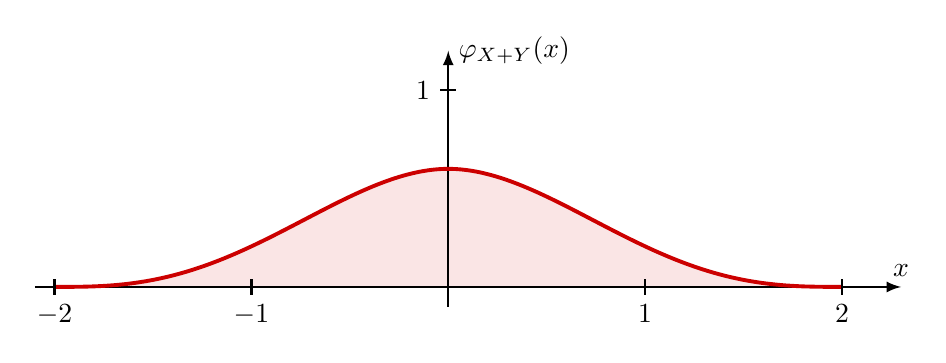
\begin{tikzpicture}[>=latex,thick]
\fill[color=darkred!10] 
	plot[domain=-2:0,samples=100]
		({\x*\h},{\h*((((3/160)*\x*\x-(3/8))*\x-(3/4))*\x*\x+3/5)})
	--
	plot[domain=0:2,samples=100]
		({\x*\h},{\h*((-((3/160)*\x*\x-(3/8))*\x-(3/4))*\x*\x+3/5)})
	-- ({2*\h},0) -- ({-2*\h},0) -- cycle;
\draw[->] ({-2.1*\h},0) -- ({2.3*\h},0) coordinate[label={$x$}];
\draw[->] (0,{-0.1*\h}) -- (0,{1.2*\h}) coordinate[label={right:$\varphi_{X+Y}(x)$}];
\draw[color=darkred,line width=1.4pt] 
	plot[domain=-2:0,samples=100]
		({\x*\h},{\h*((((3/160)*\x*\x-(3/8))*\x-(3/4))*\x*\x+3/5)})
	--
	plot[domain=0:2,samples=100]
		({\x*\h},{\h*((-((3/160)*\x*\x-(3/8))*\x-(3/4))*\x*\x+3/5)});

\foreach \x in {-2,-1,1,2}{
	\draw ({\x*\h},-0.1) -- ({\x*\h},0.1);
	\node at ({\x*\h},-0.1) [below] {$\x$};
}
\draw (-0.1,\h) -- (0.1,\h);
\node at (-0.1,\h) [left] {$1$};
\end{tikzpicture}
%\includeagraphics[]{graph-4.pdf}
\caption{Wahrscheinlichkeitsdichte $\varphi_{X+Y}(x)$ der Summe von zwei Kopien
der Zufallsvariable $X$, sie ist die Faltung der in Abbildung~\ref{50000024:dichte}
dargestellten Wahrscheinlichkeitsdichte $\varphi(x)$.
\label{50000024:summe}}
\end{figure}
\end{teilaufgaben}
\end{loesung}

